\chapter{Measurement}
\section{Units}
In this chapter of the book we are interested in how we measure length, area and volume.  We will be using the metric system which is partly based on the metre.  This metre can be divided up or multiplied to give us units like mm, cm and km.  'Milli' means ${\frac{1}{1000}}^{th}$, 'centi' means ${\frac{1}{100}}^{th}$ and 'kilo' means 1000.

\bigskip

To change m to mm we multiply by 1000 since 'milli' means ${\frac{1}{1000}}^{th}$

To change m to cm we multiply by 100 since 'centi' means ${\frac{1}{100}}^{th}$

To change m to km we divide by 1000 since 'kilo' means 1000.

\begin{exmp}
Change 3.7m into cm.

\bigskip

To change m to cm we multiply by 100.

\bigskip

So $3.7m = (3.7 \times 100) cm = 370cm$
\end{exmp}

\begin{exmp}
Change 265m into km.

\bigskip

To change m to km we divide by 1000.

\bigskip

So $265m = (265 \div 1000)km = 0.265km$

\end{exmp}
\subsection{Exercise}
Change the following lengths in 'm' to the required unit:
\begin{enumerate}
	\item $4.7m$ to $cm$
	\item $5.34m$ to $mm$
	\item $65.7m$ to $cm$
	\item $3536m$ to $km$
	\item $46m$ to $km$
	\item $362m$ to $mm$
	\item $65.3m$ to $mm$
\end{enumerate}

\section{Perimeter}
The perimeter of a shape is the length around the outside or the total of the lengths of the sides.  So if I had a triangle with sides of lengths '3m', '5m' and '4.5m' the perimiter would be $(3+5+4.5)m = 12.5m$.
\subsection{Exercise}
Find the perimeter of the following shapes:
\begin{multicols}{2}
\begin{enumerate}
	\item 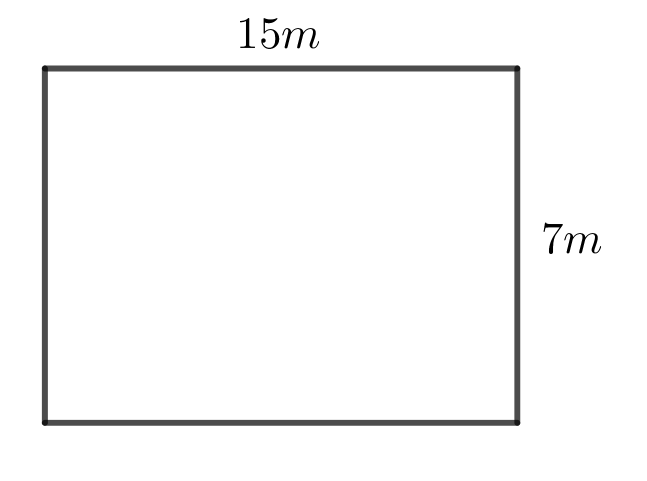
\includegraphics{./Images/Measurement/perimeter1.png}
	\item 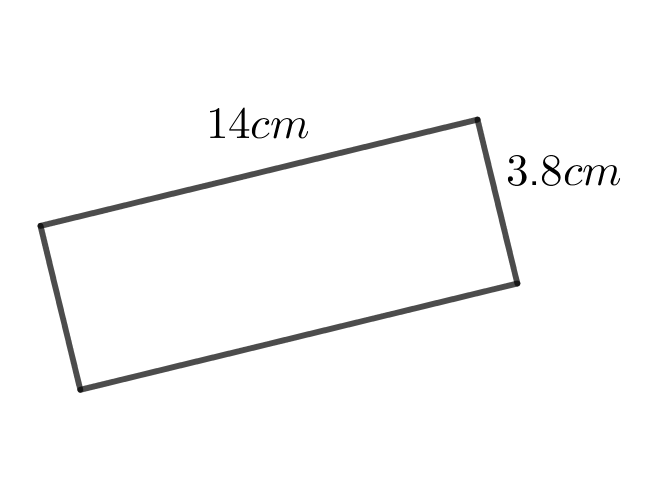
\includegraphics{./Images/Measurement/perimeter2.png}
	\item 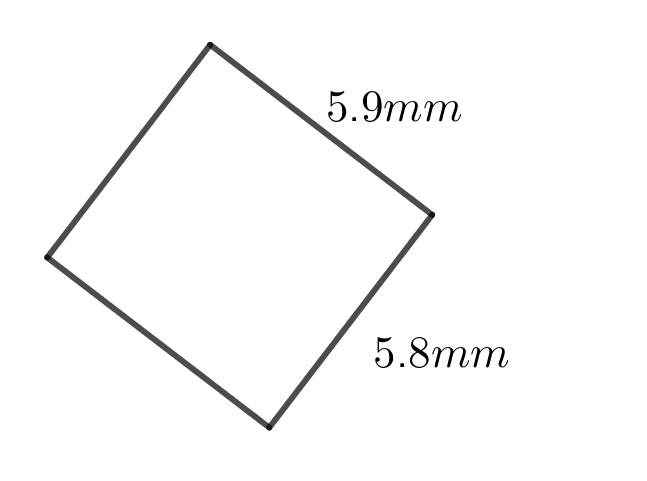
\includegraphics{./Images/Measurement/perimeter3.png}
	\item 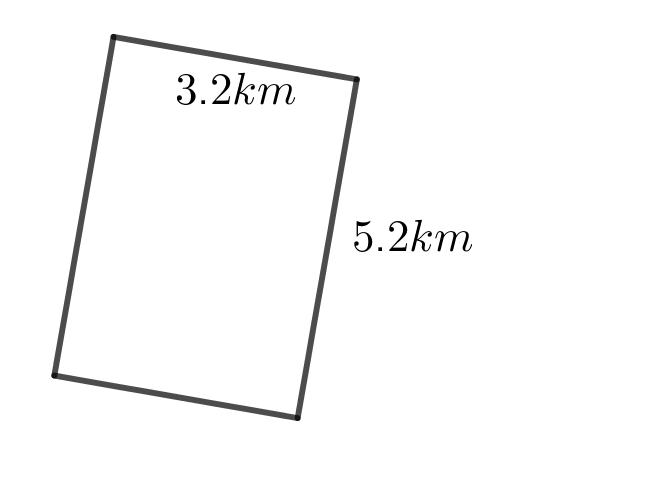
\includegraphics{./Images/Measurement/perimeter4.png}
	\item 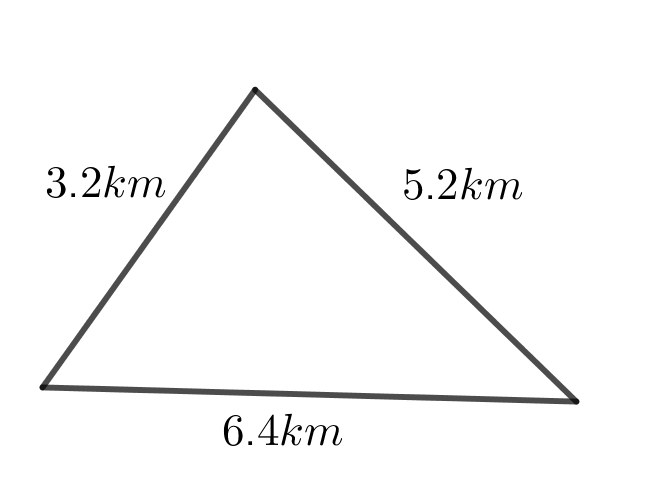
\includegraphics{./Images/Measurement/perimeter5.png}
	\item 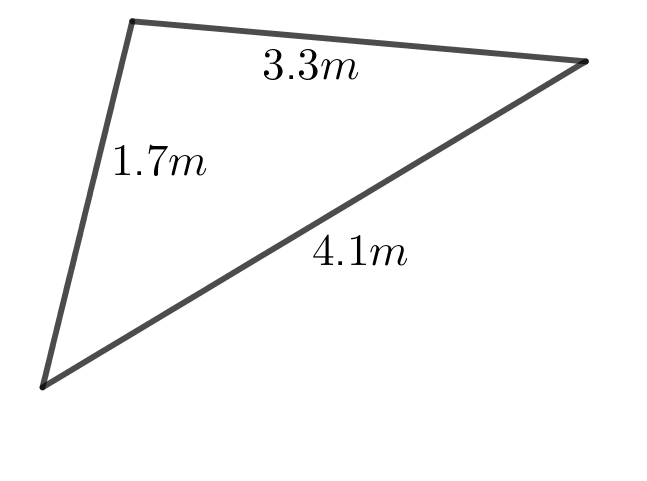
\includegraphics{./Images/Measurement/perimeter6.png}
	\item 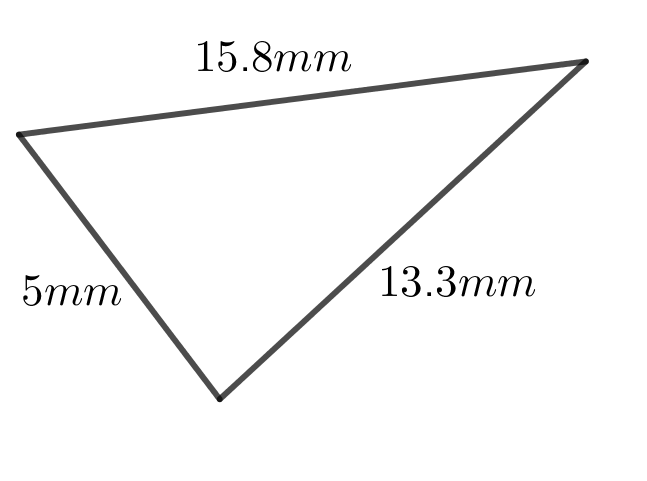
\includegraphics{./Images/Measurement/perimeter7.png}
	\item 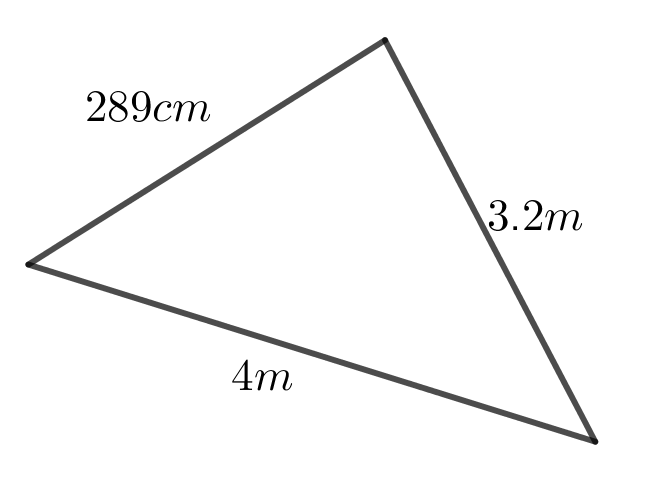
\includegraphics{./Images/Measurement/perimeter8.png}
	\item 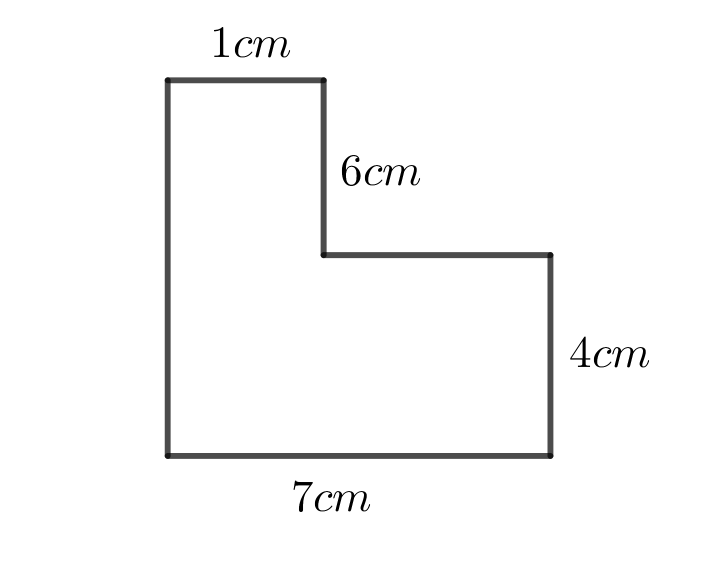
\includegraphics{./Images/Measurement/perimeter9.png}
	\item 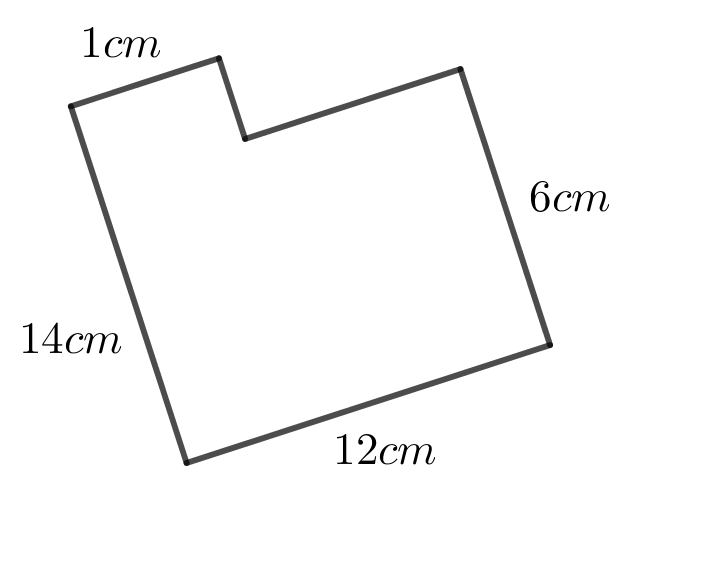
\includegraphics{./Images/Measurement/perimeter10.png}
	\item 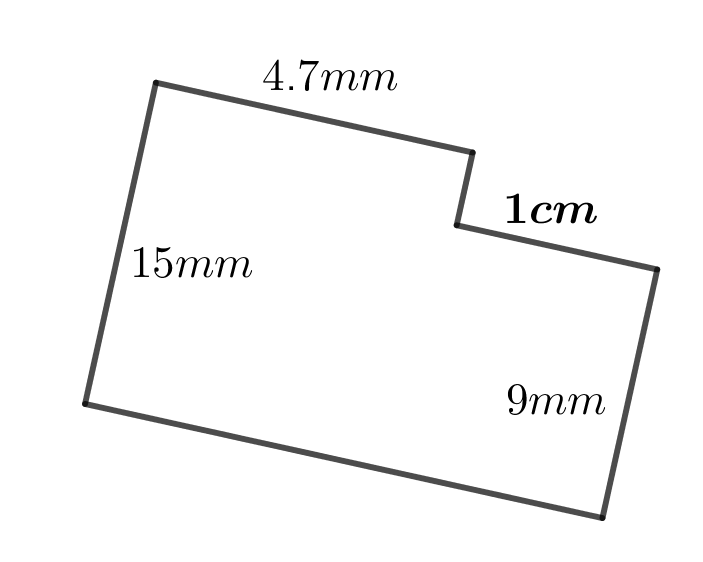
\includegraphics{./Images/Measurement/perimeter11.png}
	\item 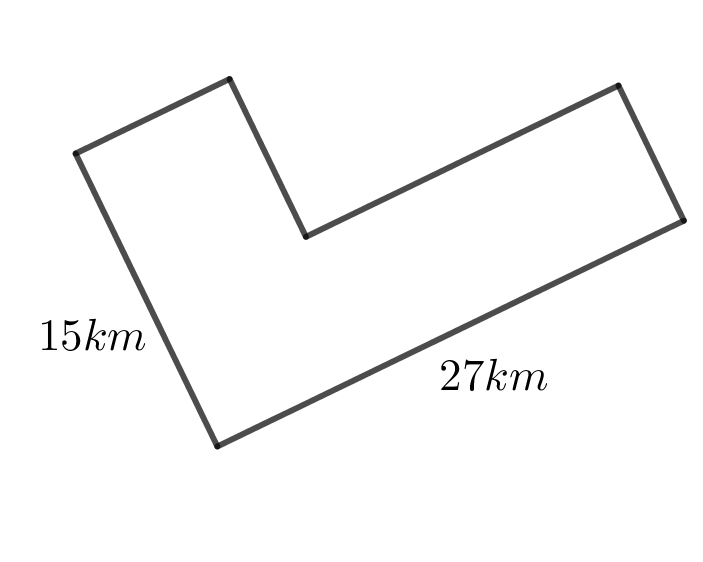
\includegraphics{./Images/Measurement/perimeter12.png}
\end{enumerate}
\end{multicols}
\subsection{Circles}
The perimeter of a circle is called the circumference.  The distance from one side of a circle to the other, through the centre, is called the diameter.  If we multiply the diameter by a particular value we can calculate the circumference.  Before I give you this value you might want to draw some circles and measure there diameters and circumferences and divide the circumference by the diameter.  When you have done that a few times continue reading.

\bigskip

If you did the exercise above, you should of got answers that were close to 3.  In fact if you managed to do it to 5 decimal places the value would have been $3.14159$.  This value is called $\pi$ which is called 'pi'.

\bigskip

To calculate the circumference of a circle we just use the formula $C=\pi d$

\begin{exmp}
Find the circumference of a circle that has a diameter of 15cm.

\bigskip

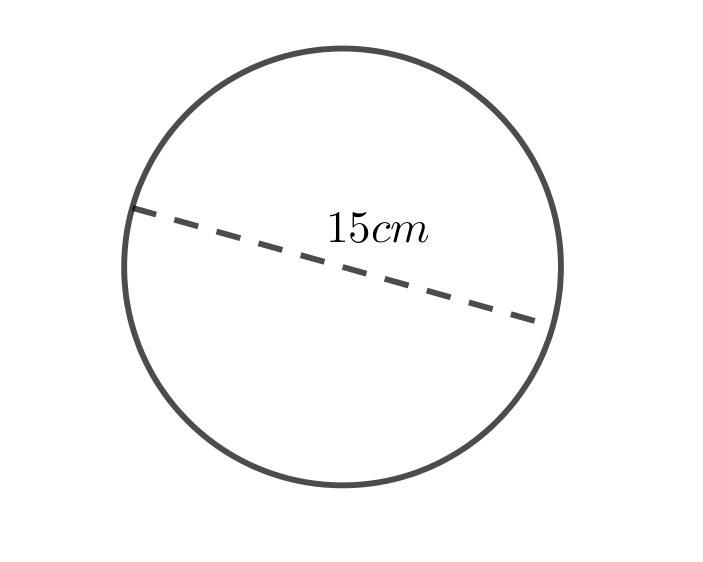
\includegraphics{./Images/Measurement/circumferenceEg1.png}

\bigskip

We know that $C=\pi d$, therefore the Circumference $=3.142 \times 15=47.13cm$
\end{exmp}

The radius of a cirle is the distance from the centre to the edge.  It follows that $C=2\pi r$
\begin{exmp}
Find the circumference of a circle that has a radius of 3.6km.

\bigskip

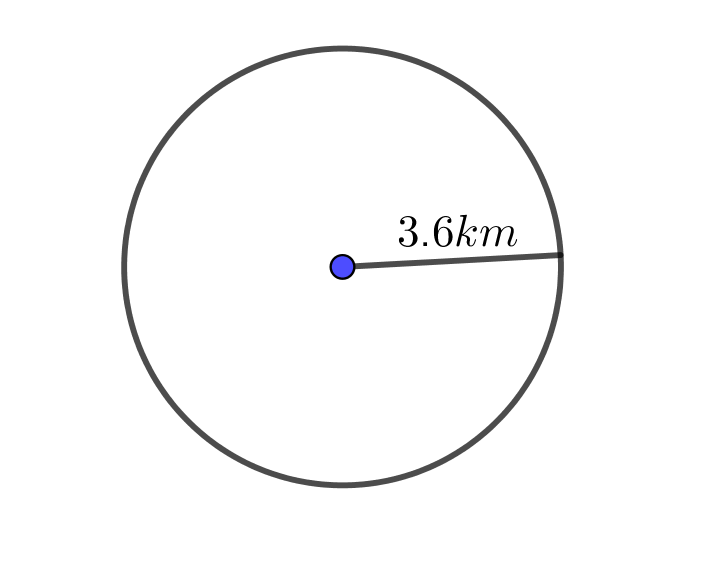
\includegraphics{./Images/Measurement/circumferenceEg2.png}

\bigskip

We know that $C=2\pi r$, therefore the Circumference $=2 \times 3.142 \times 3.6=22.622km$
\end{exmp}
\subsection{Exercise}
Find the circumference of the following circles:
\begin{enumerate}
	\item $d = 12km$
	\item $r = 6.34mm$
	\item $r = 18cm$
	\item $d = 78m$
	\item $d = 0.56mm$
	\item $r= 187km$
	\item $r = 35m$
	\item $d = 35.78m$
\end{enumerate}
\subsection{Algebraic}
\begin{exmp}
	Find $x$ given that the perimeter of the rectangle below is 58cm.

	\bigskip

	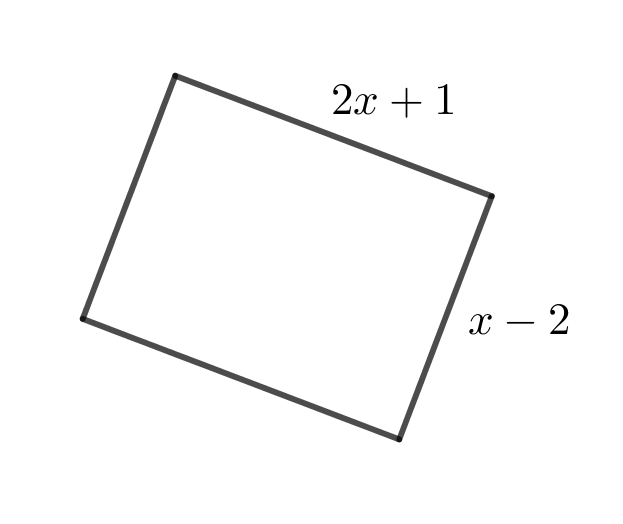
\includegraphics{./Images/Measurement/perAlgExmp1.png}

	\bigskip

	The perimeter of the shape is $2x+1+2x+1+x-2+x-2$

	\bigskip

	This simplifies to $6x-2$

	\bigskip

	Since we know the perimeter is also 58cm we can produce the equation $6x-2=58$

	\bigskip

	If we solve this equation we get $x = 10cm$

\end{exmp}

\subsection{Exercise}
Find the value of $x$ in the following:
\begin{multicols}{2}
\begin{enumerate}
	\item 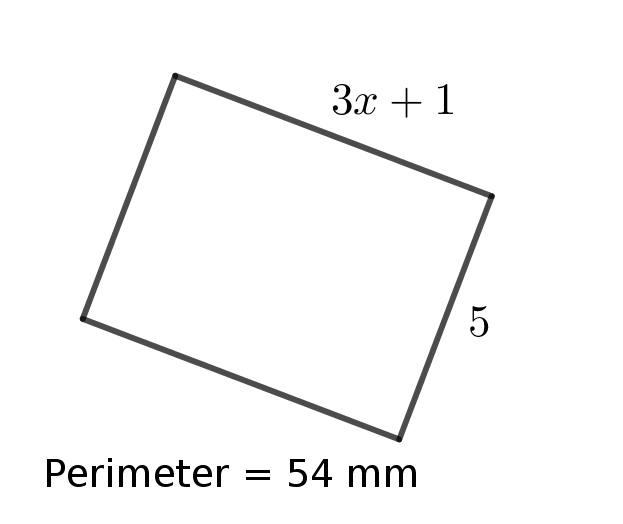
\includegraphics{./Images/Measurement/perAlg1.png}
	\item 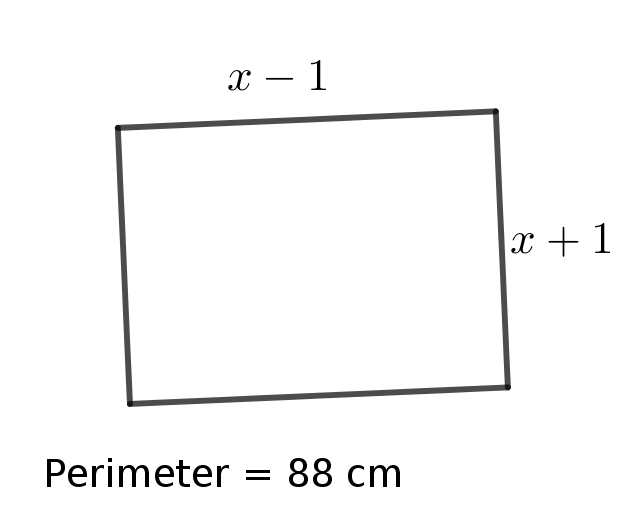
\includegraphics{./Images/Measurement/perAlg2.png}
	\item 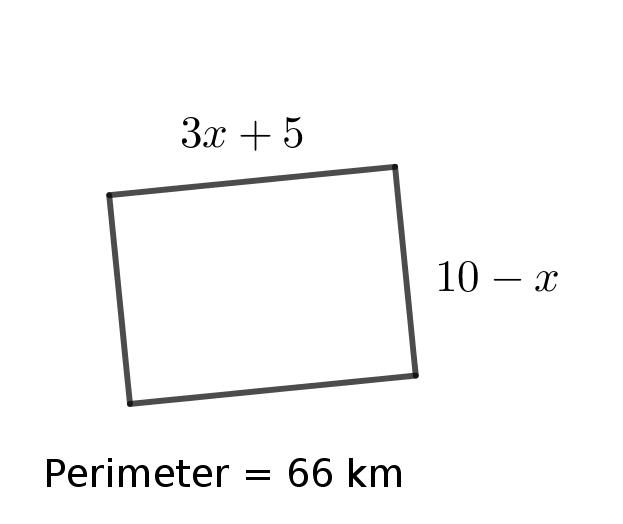
\includegraphics{./Images/Measurement/perAlg3.png}
	\item 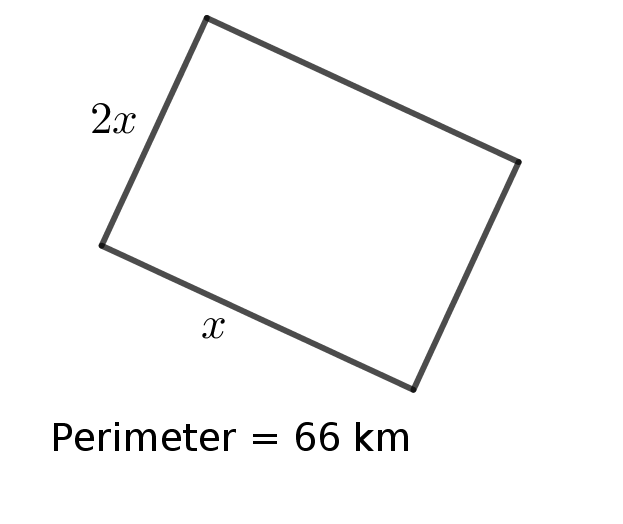
\includegraphics{./Images/Measurement/perAlg4.png}
	\item 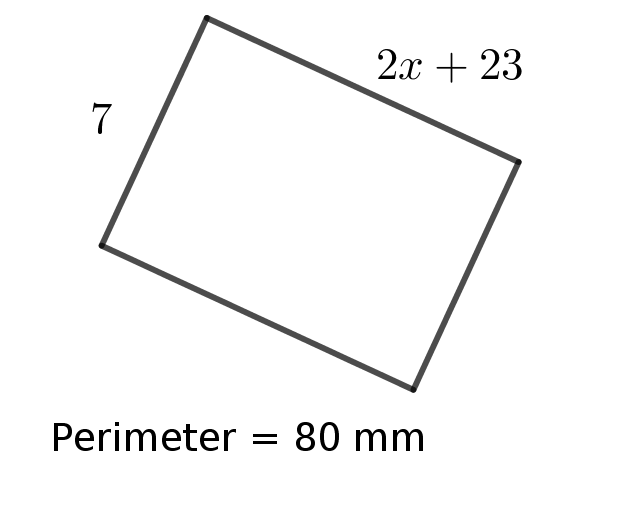
\includegraphics{./Images/Measurement/perAlg5.png}
	\item 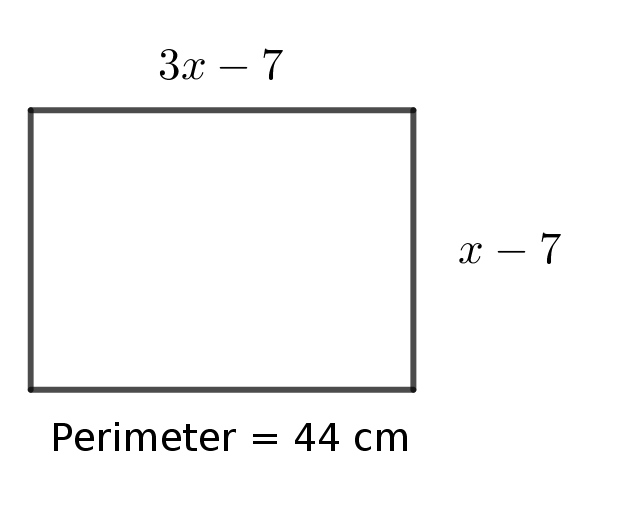
\includegraphics{./Images/Measurement/perAlg6.png}
\end{enumerate}
\end{multicols}
\section{Area}
The area of a shape is equal to the number of 1 by 1 squares that are required to cover it.

\subsubsection{Rectangle}
To calculate the area of a rectangle we multiply the length by the width.  This gives the formula:

\bigskip

$A=lw$

\begin{exmp}
	Find the area of a rectangle with a length of 7cm and a width of 10cm.

\bigskip

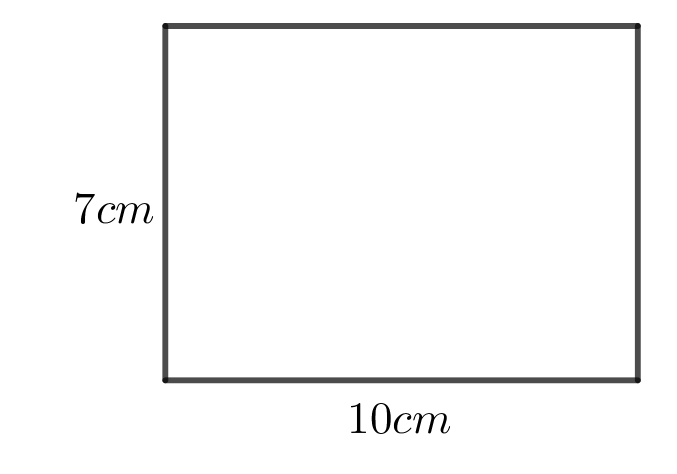
\includegraphics{./Images/Measurement/AreaEg1.png}

\bigskip

$A=lw$

\bigskip

So $A = 7 \times 10 = 70 cm^2$
\end{exmp}

\subsubsection{Triangle}
To calculate the area of a triangle we multiply the base length by the perpendicular height and divide by 2.  This gives the formula:

\bigskip

$A=\frac{bh}{2}$

\begin{exmp}
	Find the area of a triangle with a base length of 6mm and a height of 7mm.

\bigskip

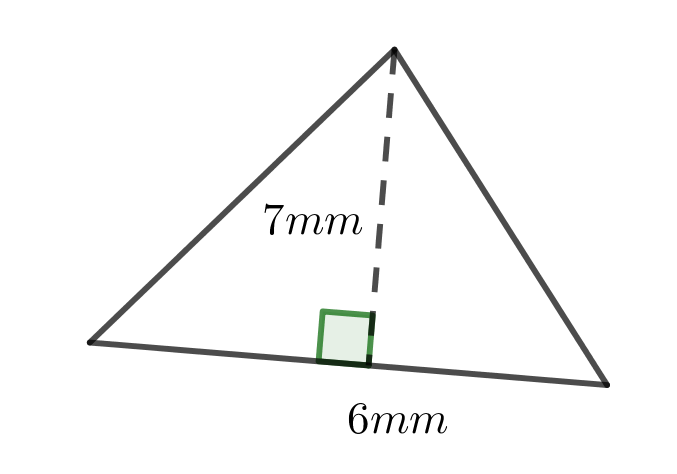
\includegraphics{./Images/Measurement/AreaEg2.png}

\bigskip

So $A = \frac{6 \times 7}{2} = 21 mm^2$
\end{exmp}
\subsubsection{Parallelogram}
To calculate the area of a parallelogram we multiply the base length by the perpendicular height.  This gives the formula:

\bigskip

$A=bh$

\begin{exmp}
	Find the area of a parallelogram which has a base length of 13 km and a perpendicular height of 5 km.

\bigskip

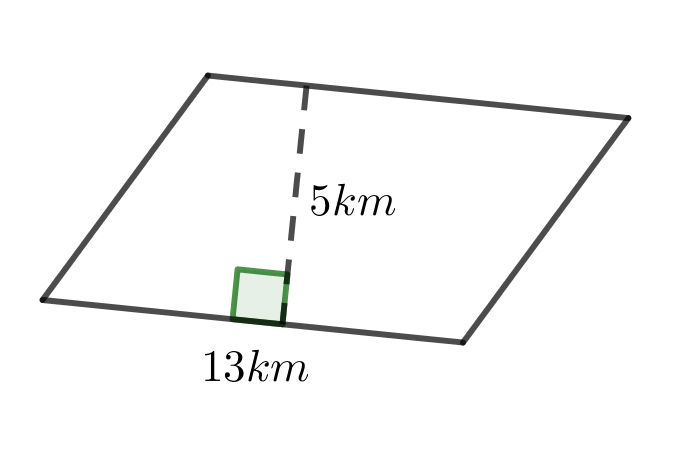
\includegraphics{./Images/Measurement/AreaEg3.png}

\bigskip

$A= 13 \times 5 = 65 km^2$
\end{exmp}

\subsubsection{Trapezium}
To calculate the area of a trapezium we multiply the average of the parallel sides by the perpendicular height (distance between them).  This gives the formula:

\bigskip

$A=\frac{(a+b)}{2}h$

\begin{exmp}
	Find the area of a trapezium which has paralell sides of lengths 6cm and 9cm and the distance between them is 8cm.

\bigskip

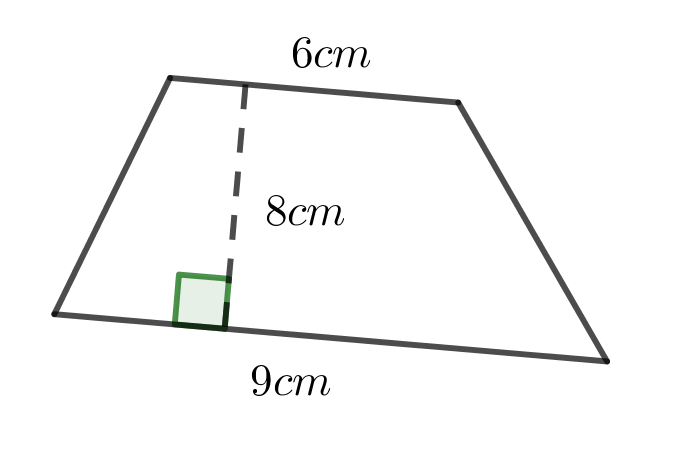
\includegraphics{./Images/Measurement/AreaEg4.png}

\bigskip

$A= \frac{(6+9)}{2}\times 8 = 60 cm^2 $
\end{exmp}

\subsection{Exercise}
Find the area of the following shapes.  Remember to show you working and include the correct units.
\begin{multicols}{2}
\begin{enumerate}
	\item 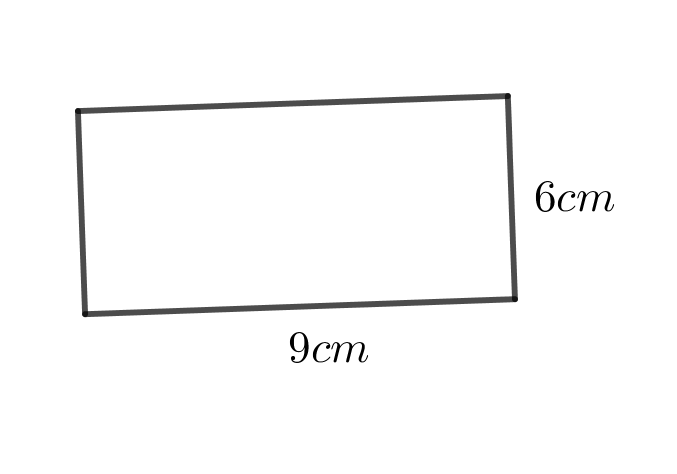
\includegraphics{./Images/Measurement/AreaQu1.png}
	\item 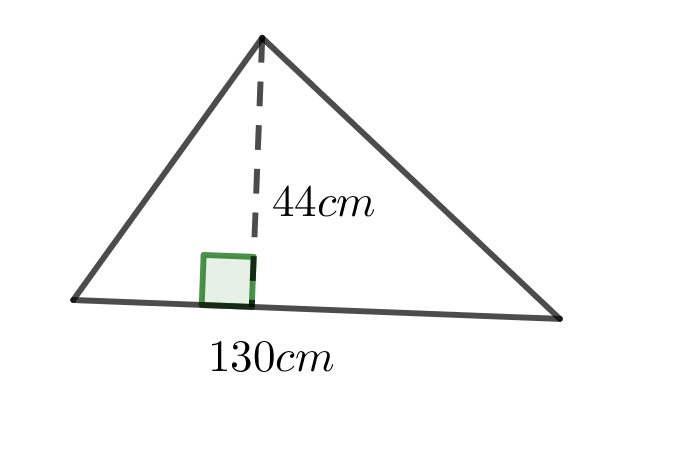
\includegraphics{./Images/Measurement/AreaQu2.png}
	\item 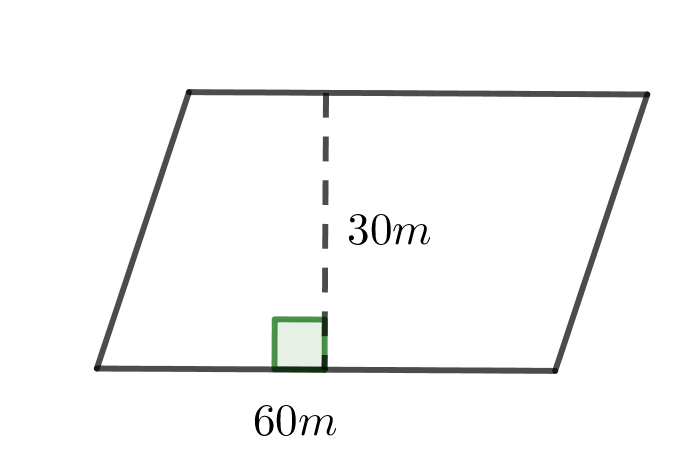
\includegraphics{./Images/Measurement/AreaQu3.png}
	\item 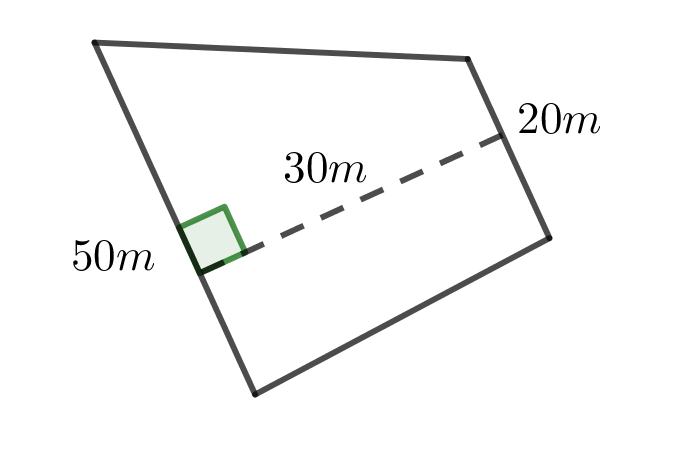
\includegraphics{./Images/Measurement/AreaQu4.png}
	\item 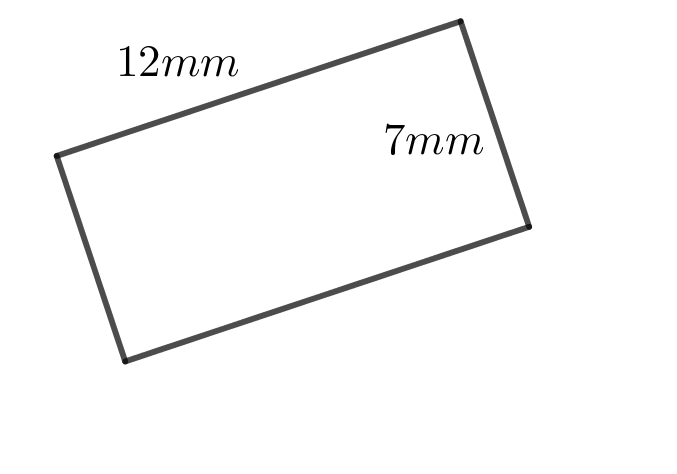
\includegraphics{./Images/Measurement/AreaQu5.png}
	\item 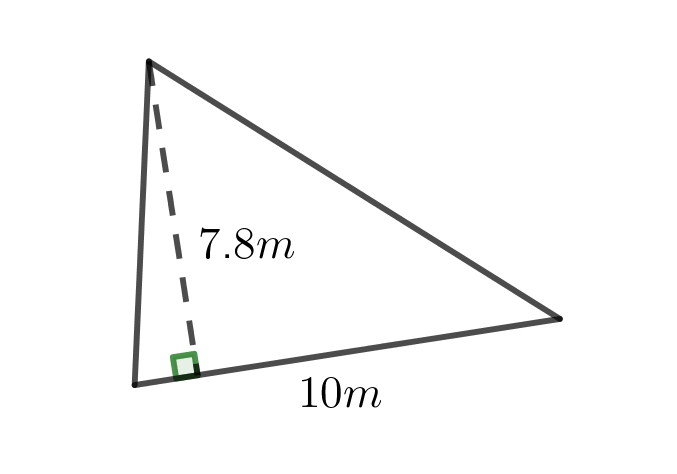
\includegraphics{./Images/Measurement/AreaQu6.png}
	\item 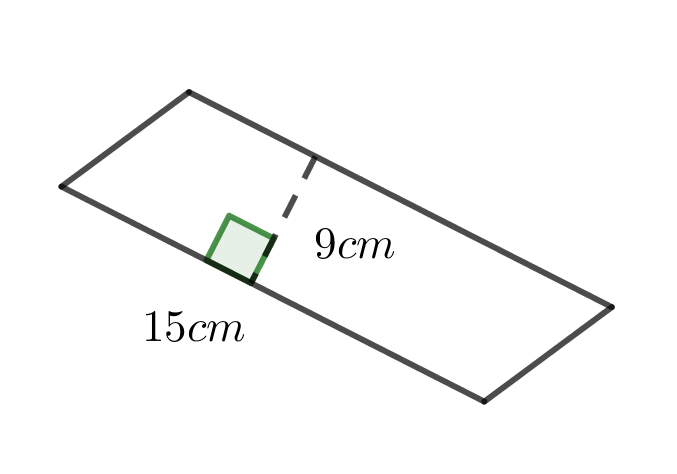
\includegraphics{./Images/Measurement/AreaQu7.png}
	\item 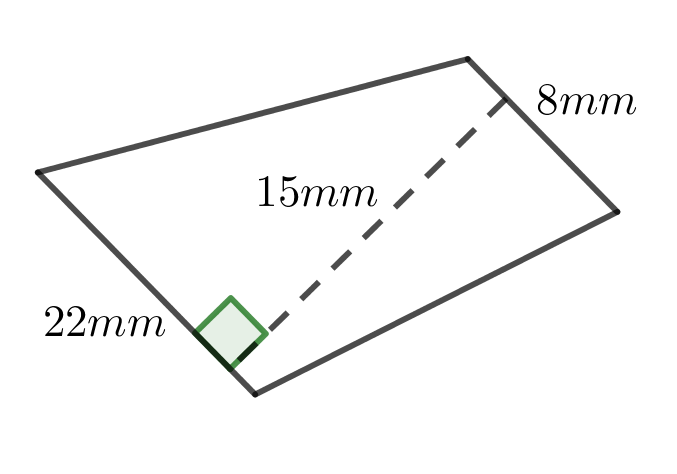
\includegraphics{./Images/Measurement/AreaQu8.png}
	\item 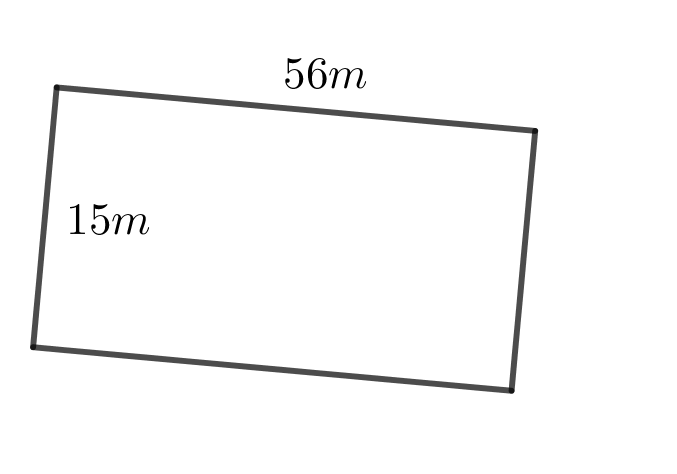
\includegraphics{./Images/Measurement/AreaQu9.png}
	\item 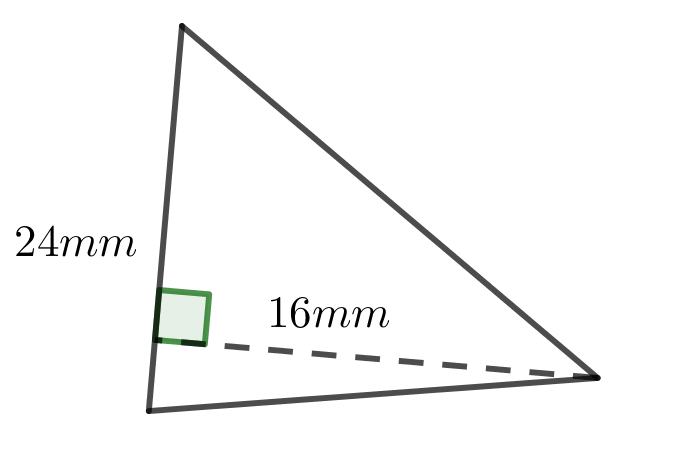
\includegraphics{./Images/Measurement/AreaQu10.png}
	\item 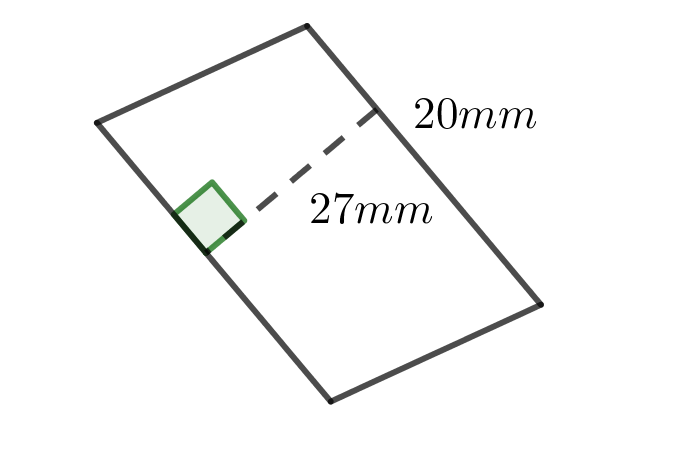
\includegraphics{./Images/Measurement/AreaQu11.png}
	\item 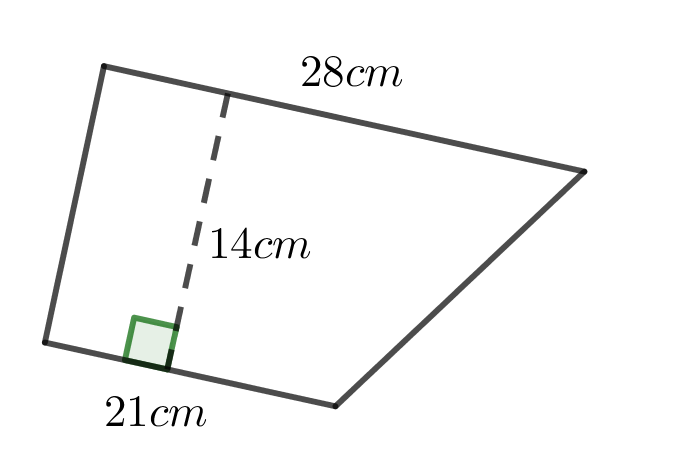
\includegraphics{./Images/Measurement/AreaQu12.png}
	\item 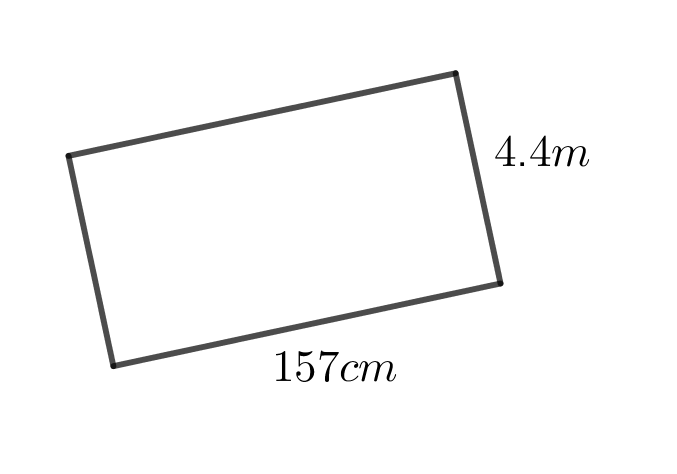
\includegraphics{./Images/Measurement/AreaQu13.png}
	\item 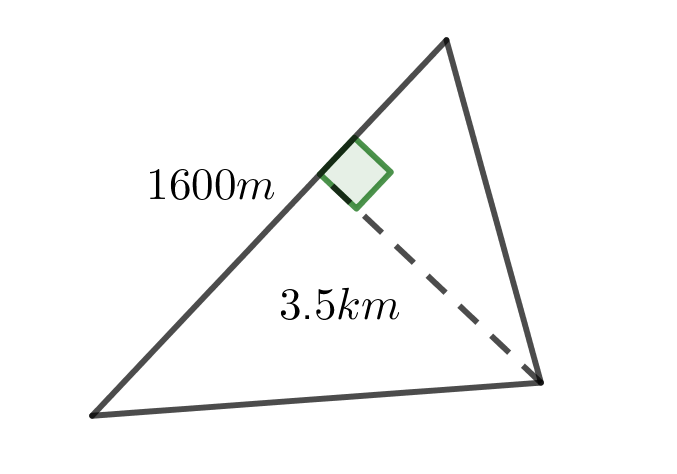
\includegraphics{./Images/Measurement/AreaQu14.png}
	\item 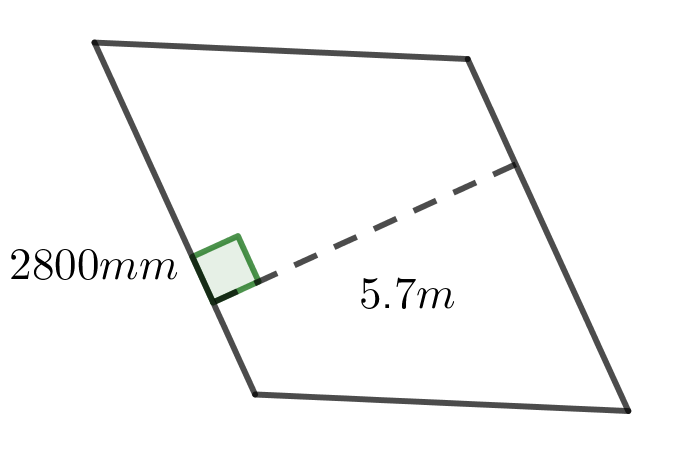
\includegraphics{./Images/Measurement/AreaQu15.png}
	\item 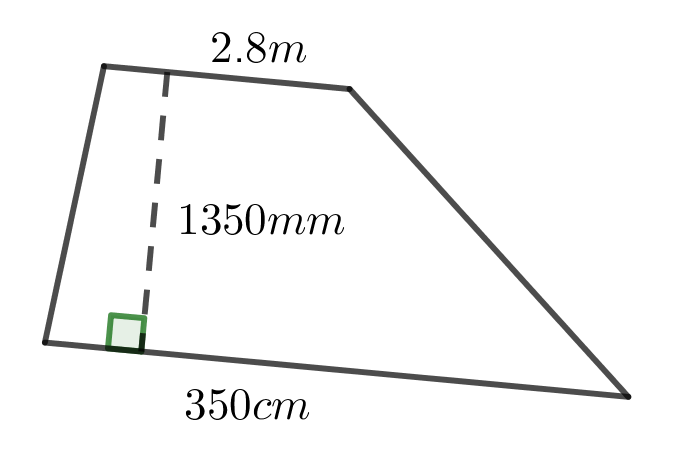
\includegraphics{./Images/Measurement/AreaQu16.png}
\end{enumerate}
\end{multicols}
\subsection{Circles}
Imagine a  circle with a radius 'r', split into sectors.

\bigskip

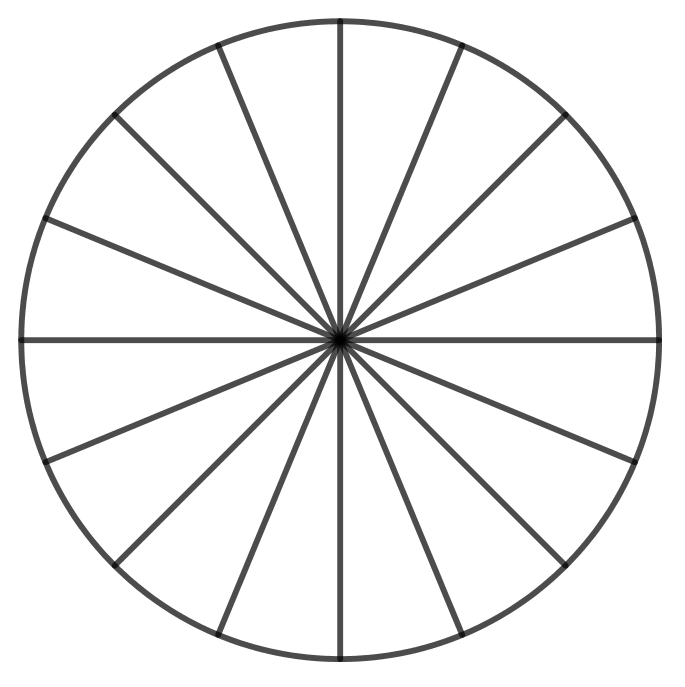
\includegraphics{./Images/Measurement/CircleSegmented.png}

\bigskip

Now rearrange the sectors as below

\bigskip

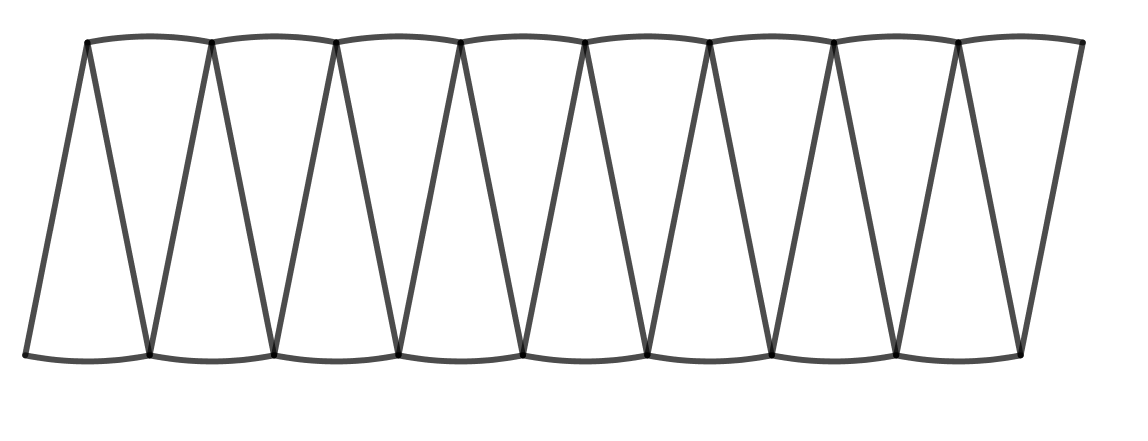
\includegraphics{./Images/Measurement/Circle2Rec.png}

The more sectors that we split our circle into the closer our rearranged shape becomes like a rectangle.  We can clearly see that this rectangle will have a height of 'r', but what is its length.  We can see that the two lengths are made up of the circumfernce of the circle which we know is $2 \pi r$, so one length would be just $\pi r$.

The area of this rectangle then would be $r \times \pi r = \pi r^2$

\bigskip

The area of a circle is found using $A=\pi r^2$

\begin{exmp}
Find the area of a circle with a radius of 5m.

\bigskip

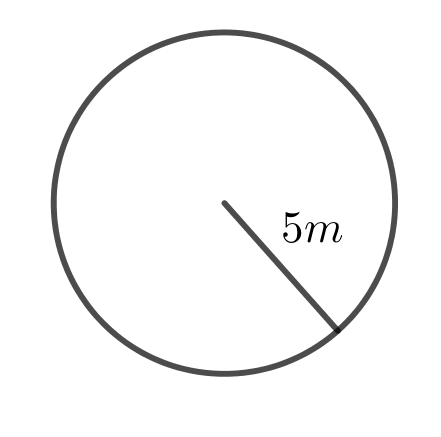
\includegraphics{./Images/Measurement/CircleAreaEg1.png}

\bigskip

So $A = \pi r^2 = \pi \times 5^2 = 78.54 m^2$


\end{exmp}

\begin{exmp}
Find the area of a circle with a diameter of 8.6mm.

\bigskip

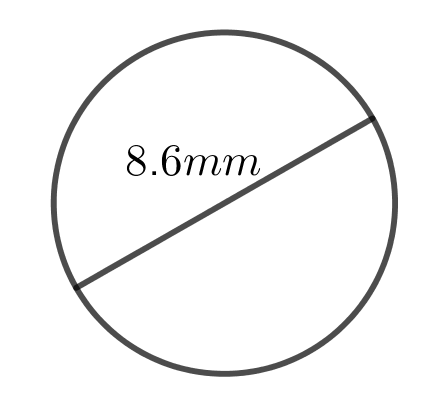
\includegraphics{./Images/Measurement/CircleAreaEg2.png}

\bigskip

The radius is half the diameter so the radius is 4.3mm.

\bigskip

So $A = \pi r^2 = \pi \times 4.3^2 = 58.1 mm^2$

\end{exmp}

\subsection{Exercise}
Find the areas of the following circles, make sure you include the units.
\begin{multicols}{2}
\begin{enumerate}
	\item 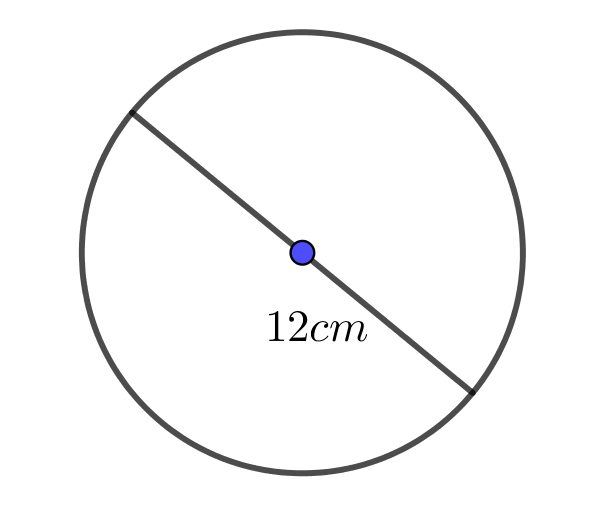
\includegraphics{./Images/Measurement/CircleAreaEx1.png}
	\item 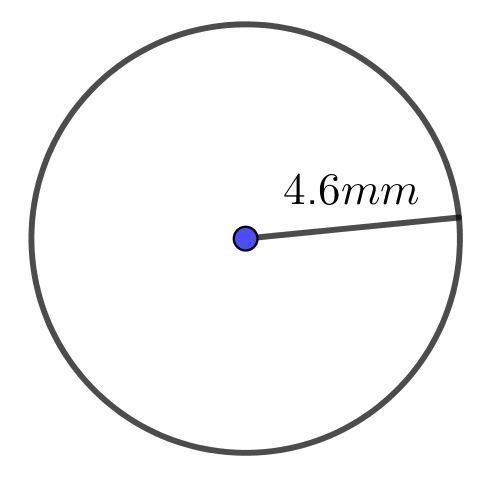
\includegraphics{./Images/Measurement/CircleAreaEx2.png}
	\item 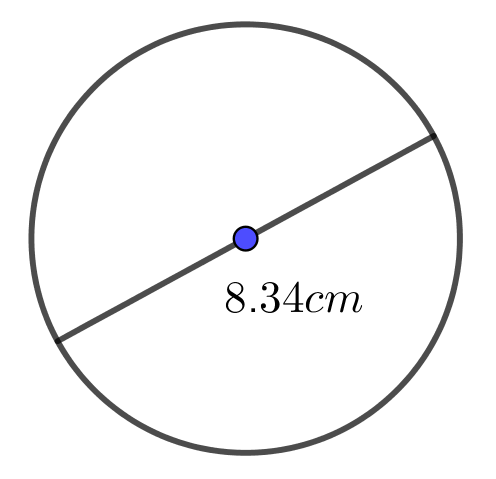
\includegraphics{./Images/Measurement/CircleAreaEx3.png}
	\item 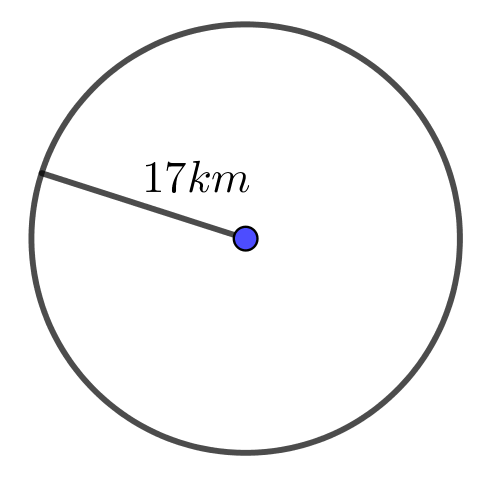
\includegraphics{./Images/Measurement/CircleAreaEx4.png}
	\item 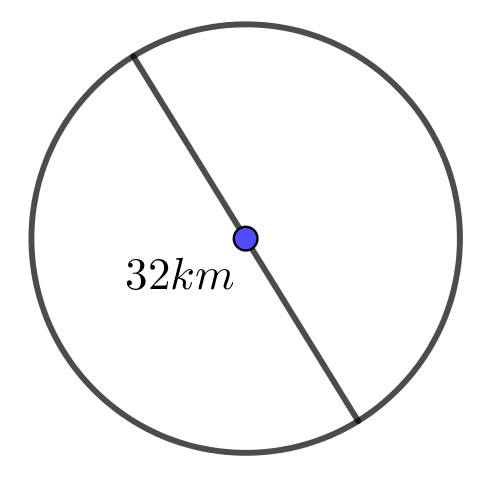
\includegraphics{./Images/Measurement/CircleAreaEx5.png}
	\item \includegraphics{./Images/Measurement/CircleAreaEx6.png}
\end{enumerate}
\end{multicols}

\subsection{Surface Area}
The surface area of a shape is equal to the total of the areas of it various surfaces.  Normally we would work this out by sketching each of the surfaces as if they were flat, work out their individual areas and then add them.  We will look at the special cases of cuboids, cylinders and spheres and then look at some examples of 'odd' shapes.
\subsubsection{Cuboids}
A cuboid is like a box.

\bigskip

\includegraphics{./Images/Measurement/CuboidPic.png}

\bigskip

Opposite faces are identical, so it is made up three pairs of faces.

If we have a cuboid which is $l \times w \times h$ then the three faces will be:

\begin{itemize}
	\item $l \times w$
	\item $l \times h$
	\item $w \times h$
\end{itemize}

We can work each of these areas out add them together and multiply the answer by 2.

\begin{exmp}
Find the surface area of the cuboid below:

\bigskip

\includegraphics{./Images/Measurement/CuboidEg.png}

\bigskip

First we change the lengths all to the same unit, I will choose $m$.  So we have a $2m \times 1.2m \times 0.85m$ cuboid.

The three faces are:

\begin{itemize}
	\item $2 \times 1.2 = 2.4m^2$
	\item $2 \times 0.85 = 1.7m^2$
	\item $1.2 \times 0.85 \approx 1m^2$
\end{itemize}

The surface area is $2 \times (2.4 + 1.7 + 1)=10.2m^2$
\end{exmp}

\subsubsection{Cylinder}
A cylinder is made up of two identical circls joined by a curved rectangle.

\bigskip

\includegraphics{./Images/Measurement/CylinderNet.png}

\bigskip

To calculate the area of the circles we need their radius to work out the area of the rectangle we need the rectangles height and width.  Since the rectangle is curved around the circles its width must equal the circumference of the circle, so we can use $2 \pi r$ to obtain the width of the rectangle.

\begin{exmp}
Find the surface area of the cylinder below:

\bigskip

\includegraphics{./Images/Measurement/CylinderEg.png}

\bigskip

The circles have a radius of $4cm$, so the area of each circle is $\pi \times 4^2 = 50.27cm^2$

The circumference of a circle is $2 \times \pi \times 4 = 25.13cm$, so the area of the rectangle is $25.13 \times 7 = 175.9cm^2$

Therefore the surface area is $2 \times 50.27 + 175.9 = 276.5cm^2$

\end{exmp}


\subsubsection{Sphere}
The surface area of a sphere is calculated with the formula $A = 4 \pi r^2$

\begin{exmp}
Find the surface area of a sphere with a diameter of $10cm$.

The radius is $5cm$, so the surface area is $4 \times \pi \times 5^2=314cm^2$
\end{exmp}

\subsubsection{Odd shapes}
Here we find teh area of each face no matter what shape it is and add the values together.

\begin{exmp}
Find the surface area of the shape below:

\bigskip

\includegraphics{./Images/Measurement/OddSA.png}

\bigskip

We have a total of 8 faces (6 rectangles and 2 'L' shapes)

Three of the rectangles have areas of $1 \times 5 = 5cm^2$
Two of the rectangles have areas of $2 \times 5 = 10cm^2$
One  of the rectangles have areas of $3 \times 5 = 15cm^2$
The two 'L' shapes have areas of $4cm^2$

That gives a total surface area of $58cm^2$
\end{exmp}
\subsection{Exercise}
Find the surface area of the following shapes:

\subsection{Expanding Brackets}
When we talk about expanding brackets we mean multiplying a bracket by a a term or another bracket.  We can get questions in the form:

Expand $5(x+7)$  or $(x-4)(x+6)$

We are going to use the areas of rectangles to show how this works.

Let's consider $4(3+4)$.  We can see quite easily that the answer to this is 28 using BEDMAS.  Now let's look at the rectangle that represents this situation.

\bigskip

\includegraphics{./Images/Measurement/ExpandBrackets1.png}

\bigskip

The area of A is 12 and the area of B is 16, so the total is 28.  It should be noted that we did this by multiplying the 4 by 3 and the 4 by 4.

\bigskip

Now let's consider $x(x+6)$

\bigskip

\includegraphics{./Images/Measurement/ExpandBrackets2.png}

\bigskip

Here area A is $x^2$

\bigskip

The area of B is $6x$

\bigskip

So the total area is $x^2+6x$.  We got this by multiplying the $x$ by both terms in the bracket.

\bigskip

Now let's consider $x(x-3)$

\bigskip

\includegraphics{./Images/Measurement/ExpandBrackets3.png}

\bigskip

Rectangle A has a length of $x-3$ and a height of $x$ so this is the area we require.

\bigskip

The total area is $x^2$, the area of B is $3x$

\bigskip

So the required area is $x^2 - 3x$.  Again we multiplied the $x$ on the outside with all the terms within the bracket.

\bigskip

Finally, let's consider $(x+5)(x+3)$

\bigskip

\includegraphics{./Images/Measurement/ExpandBrackets4.png}

\bigskip

The area of A is $x^2$, the area of B is $3x$, the area of C is $5x$ and the area of D is $15$

\bigskip

So the total area is $x^2 + 8x + 15$ which is the expansion of $(x+5)(x+3)$

\begin{exmp}
Expand $(x+2)(2x-5)$

\bigskip

We multiply each term in the first bracket by each term in the second bracket.

\bigskip

$(x+2)(2x-5)=2x^2-5x+2x-10$

So $(x+2)(2x-5)=2x^2-3x-10$
\end{exmp}

\subsection{Exercise}
Expand and simplify each of the expressions below:
\begin{multicols}{3}
\begin{enumerate}
	\item $4(x+7)$
	\item $9(6-x)$
	\item $x(x+5)$
	\item $4(x+y)$
	\item $x(x-y)$
	\item $x(x+y+z)$
	\item $3x(x+2)$
	\item $5x(3x-4)$
	\item $(x+2)(x+5)$
	\item $(p+7)(p+4)$
	\item $(t+4)(t+3)$
	\item $(d+5)(d+6)$
	\item $(x+5(x-4)$
	\item $(y-6)(y+3)$
	\item $(t+2)(t-2)$
	\item $(g+10)(g-10)$
	\item $(2x+4)(x+7)$
	\item $(3x-7)(2x+4$
	\item $(5x-3)(x-5)$
	\item $(3t-5)(3t+1)$
	\item $(t-4)^2$
	\item $(4-t)^2$
	\item $(2x+3)^2$
	\item $(x+y)^2$
\end{enumerate}
\end{multicols}

\section{Volume}
When we are finding the volume of a shape we are calculating the number of unit cubes that will fit in it.
